\section{Implementation}
\label{Imp}

We run modified contiki-ng, a system for next generation IOT (Internet of things), on data plane. we modified the network layer of contiki-ng, and abstract data plane interface to separate network control functions from data plane. 

Neighbor discovery, After deployment, nodes start IPv6 neighbor discovery protocol to find the nodes which communicate with it within one hop, and save neighbor information to neighbor table and wait for UAV arrive 
and gather the topology information. Every neighbor's information include the neighbor's IP and RSSI. 

Packet forwarding, the nodes get routing table from UAV through northbound interface, when it receive a data packet from other nodes, it just send it to the next hop node according the routing table.

Data sampling, node read task table received from UAV to decide when to wake up sensors to make sure node cost minimal energy to get same quality data. 

On UAV, we run our UAV flight controller on ROS and use MySQL as our SDN database, UAV gathered topology data from every node and save in database, 
so user can easily read the whole network data from database, For the same 
reasoning, after user get routing algorithm result and save it to database via northbound interface, 
our middleware will automatically divide the whole network routing result to individual node routing table, and then send it to specific node.

\begin{figure}[htbp]
	\centering
	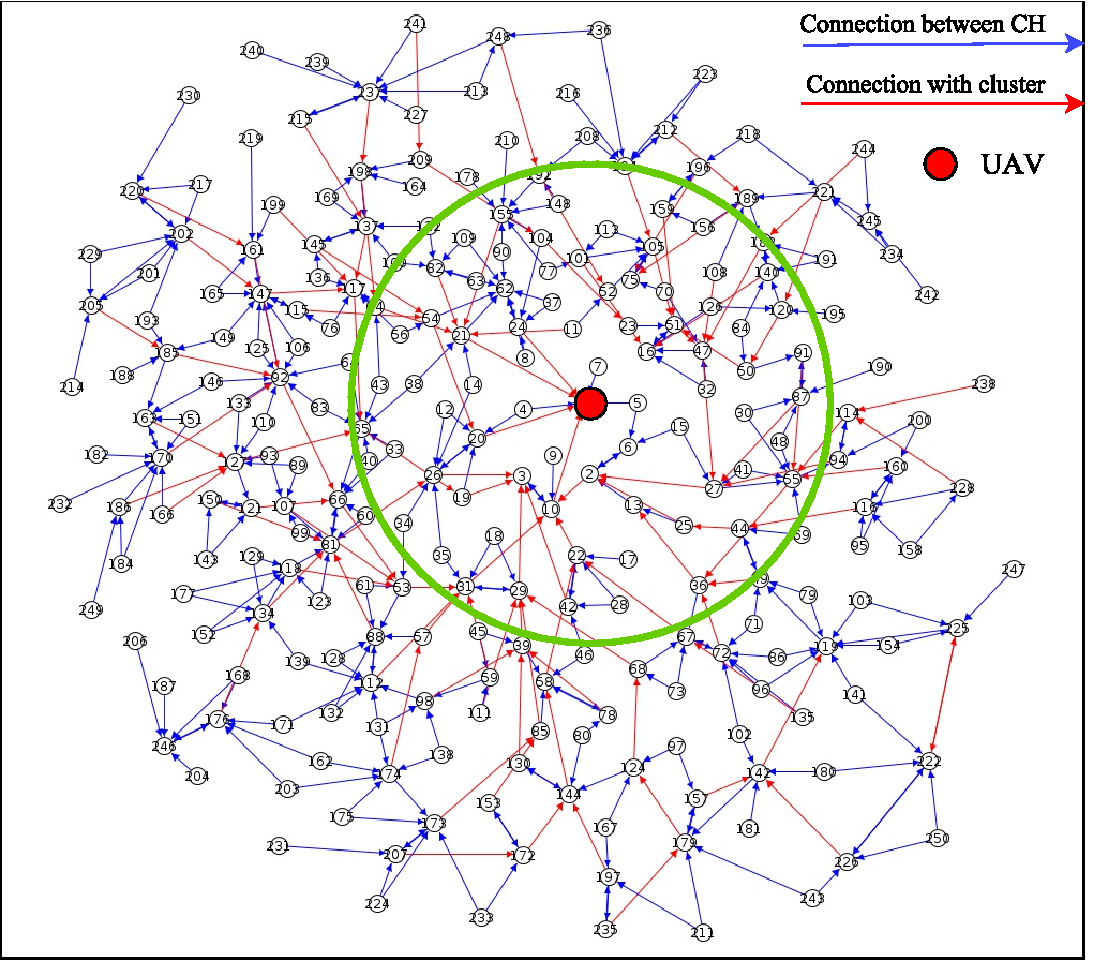
\includegraphics[width=.85\columnwidth]{Figure/topology}
	\vspace{-0.1in}
	\caption{Network topology}
	\label{routing-flow}
	\vspace{-0.1in}
\end{figure}

